\RequirePackage{plautopatch}
\documentclass[uplatex,dvipdfmx,a4paper,10pt]{jsarticle}
\usepackage{graphicx}
\usepackage{amsmath}
\usepackage{csvsimple}
\usepackage{dcolumn}
\usepackage{siunitx}
\usepackage{url}

\title{電気回路}
\author{電気通信大学 I\hspace{-1.2pt}I\hspace{-1.2pt}I類\\
2313213 山口海音}
\date{\today 作成}

\begin{document}
\maketitle

\section{目的}
RLC直列回路を作成し，電流の減衰振動，過減衰を観測することで，その周波数やピーク電圧を計算値と比較し，考慮できていないインピーダンスを考える．

\section{原理}

抵抗値$R$の抵抗による電圧降下は，オームの法則から$V_\mathrm{R} = RI$であり，誘導係数$L$のコイルによる電圧降下は$V_\mathrm{L} = L\dot{I}$\footnote{電気回路の分野において物理量$X$に対して，$\dot{X}$はその物理量のベクトル表示，$X$はその大きさを表すことが多いが，このレポートにおいては，$\dot{X}$はその物理量の時間微分を表すこととする．}であり，静電容量$C$のコンデンサによる電圧降下は$V_\mathrm{C} = \dfrac{1}{C}Q$である．起電力と電圧降下が等しいことから
\begin{equation}
    V = L\dot{I} + RI + \frac{1}{C}Q
\end{equation}
が成り立ち，これを時間微分することで
\begin{equation}
    0 = L\ddot{I} + R\dot{I} + \frac{1}{C}I
\end{equation}
を得るが，$\gamma=\dfrac{R}{2L}$，$\omega=\dfrac{1}{\sqrt{LC}}$とすると
\begin{equation}\label{current-eq}
    0 = \ddot{I} + 2\gamma \dot{I} + \omega^2I
\end{equation}
と表せる．この方程式の解は，$\gamma$と$\omega$の大きさに依る．

\subsection{臨界減衰}\label{sec:LD}
$\gamma = \omega$のとき，$I_0=I(t=0)$，$\dot{I}_0=\dot{I}(t=0)$とすると，式\ref{current-eq}の解は，
\begin{align}
    I &= e^{-\gamma t}\left( I_0 + \left( \dot{I}_0+\gamma I_0 \right)t\right)
\end{align}
である．

\subsection{減衰振動}\label{sec:DO}
$\gamma < \omega$のとき，$\omega'=\sqrt{\omega^2 - \gamma^2}$，$I_0=I(t=0)$，$\dot{I}_0=\dot{I}(t=0)$，$e^a=A=\sqrt{\left( {\dfrac{\dot{I}_0+\gamma I_0}{\omega'}} \right)^2 + {I_0}^2}$とし，$\theta$を$\sin{\theta}=\dfrac{I_0}{A}$，$\cos{\theta}=\dfrac{\dot{I}_0+\gamma I_0}{\omega'A}$を満たす実数とすると，式\ref{current-eq}の解は，
\begin{align}
    I &= e^{-\gamma t}\left( I_0\cos{\omega't} + \dfrac{\dot{I}_0+\gamma I_0}{\omega'}\sin{\omega't}\right)\\
    &= e^{-\gamma t + a} \sin\left( \omega't + \theta \right)
\end{align}
である．$\Delta\theta$を$\sin{\left( -\Delta\theta \right)}=-\dfrac{\omega'}{\omega}$，$\cos{\left( -\Delta\theta \right)}=\dfrac{\gamma}{\omega}$を満たす実数とし，$I$を時間微分すると，
\begin{align}
    \dot{I} &= \omega' e^{-\gamma t + a} \cos\left( \omega't + \theta \right) -\gamma e^{-\gamma t + a} \sin\left( \omega't + \theta \right)\\
    &= -e^{-\gamma t + a + \ln{\omega}} \sin\left( \omega't + \theta - \Delta\theta\right)
\end{align}
となるため，$I$は，$\dot{I}=0$となるとき，即ち，
\begin{equation}
    \omega't + \theta = \Delta\theta + n\pi
\end{equation}
となるときにピークを迎える．このような時間$t$を$t_n$とし，このときの電流$I$を$I_n$とすると，$t_n = \dfrac{1}{\omega'}\left( -\theta + \Delta\theta + n\pi \right)$，$I_n = (-1)^n e^{-\gamma t_n + a} \sin \Delta\theta $となる．よって$I$は$\dfrac{\pi}{\omega'}$毎にピークを迎える，即ち，周期性があることがわかり，そのピーク電圧の大きさは
\begin{equation}\label{I-strength}
    |I_n| = e^{-\gamma t_n + a}\sin \Delta\theta
\end{equation}で与えられる．

実験では，オームの法則から電流$I$と比例関係にある抵抗器の端子電圧$V_\mathrm{R}$の波形をオシロスコープで見て，極大または極小の間隔から周期$T_\mathrm{exp}$を求め，そこにおける電圧強度の割合の変化から$\gamma$を求める．

$V_n=RI_n$は，
\begin{equation}
    |V_n| = e^{-\gamma t_n + a}R\sin \Delta\theta
\end{equation}
を満たすが，この対数を取ると，
\begin{equation}
    \ln{|V_n|} = -\gamma t_n + a + \ln{R} + \ln{\sin\Delta\theta}
\end{equation}
となり，$\ln{|V_n|}$と$t_n$の関係が一次関数で表される．$\gamma$を求める上でこれは都合がよい．

\subsection{過減衰}\label{sec:OD}
$\gamma > \omega$のとき，$\omega'=\sqrt{\gamma^2 - \omega^2}$，$I_0=I(t=0)$，$\dot{I}_0=\dot{I}(t=0)$，$e^a=A=\sqrt{\left( {\dfrac{\dot{I}_0+\gamma I_0}{\omega'}} \right)^2 - {I_0}^2}$とし，$\theta$を$\sinh{\theta}=\dfrac{I_0}{A}$，$\cosh{\theta}=\dfrac{\dot{I}_0+\gamma I_0}{\omega'A}$を満たす実数とすると，式\ref{current-eq}の解は，
\begin{align}
    I &= e^{-\gamma t}\left( I_0\cosh{\omega't} + \dfrac{\dot{I}_0+\gamma I_0}{\omega'}\sinh{\omega't}\right)\\
    &= e^{-\gamma t + a} \sinh\left( \omega't + \theta \right)
\end{align}
である．$\Delta\theta$を$\sinh{\left( -\Delta\theta \right)}=-\dfrac{\omega'}{\omega}$，$\cosh{\left( -\Delta\theta \right)}=\dfrac{\gamma}{\omega}$を満たす実数とし，$I$を時間微分すると，
\begin{align}
    \dot{I} &= \omega' e^{-\gamma t + a} \cosh\left( \omega't + \theta \right) - \gamma e^{-\gamma t + a} \sinh\left( \omega't + \theta \right)\\
    &= -e^{-\gamma t + a + \ln{\omega}} \sinh\left( \omega't + \theta - \Delta\theta\right)
\end{align}
となるため，$I$は，$\dot{I}=0$となるとき，即ち，
\begin{equation}
    \omega't + \theta = \Delta\theta
\end{equation}
となるときにピークを迎える．このような時間$t$を$t_0$とし，このときの電流$I$を$I_0$とすると，$t_0 = \dfrac{1}{\omega'}\left( -\theta + \Delta\theta\right)$，$I_n = (-1)^n e^{-\gamma t_0 + a} \sin \Delta\theta $となる．

実験では，オームの法則から電流$I$と比例関係にある抵抗器の端子電圧$V_\mathrm{R}$の波形をオシロスコープで見て，一定時間$\Delta T$毎の電圧強度の割合の変化を見て，減衰振動の場合と比べる．

$V=RI$は，
\begin{equation}
    V = e^{-\gamma t + a} \sinh\left( \omega't + \theta \right)
\end{equation}
を満たすが，この対数を取ると，
\begin{equation}
    \ln{V} = -\gamma t_n + a + \ln{\sinh\left( \omega't + \theta \right)}
\end{equation}
となり，$\ln{V}$と$t_n$の関係が一次関数では表されず．減衰振動の場合と比べてグラフが直線よりも歪むことになる．

\section{実験方法}

図\ref{circuit}のような回路を作成し，抵抗器の端子間電圧$V_\mathrm{R}$を測定することで電流$I$を間接的に観測する．
\begin{figure}[htbp]
    \begin{center}
        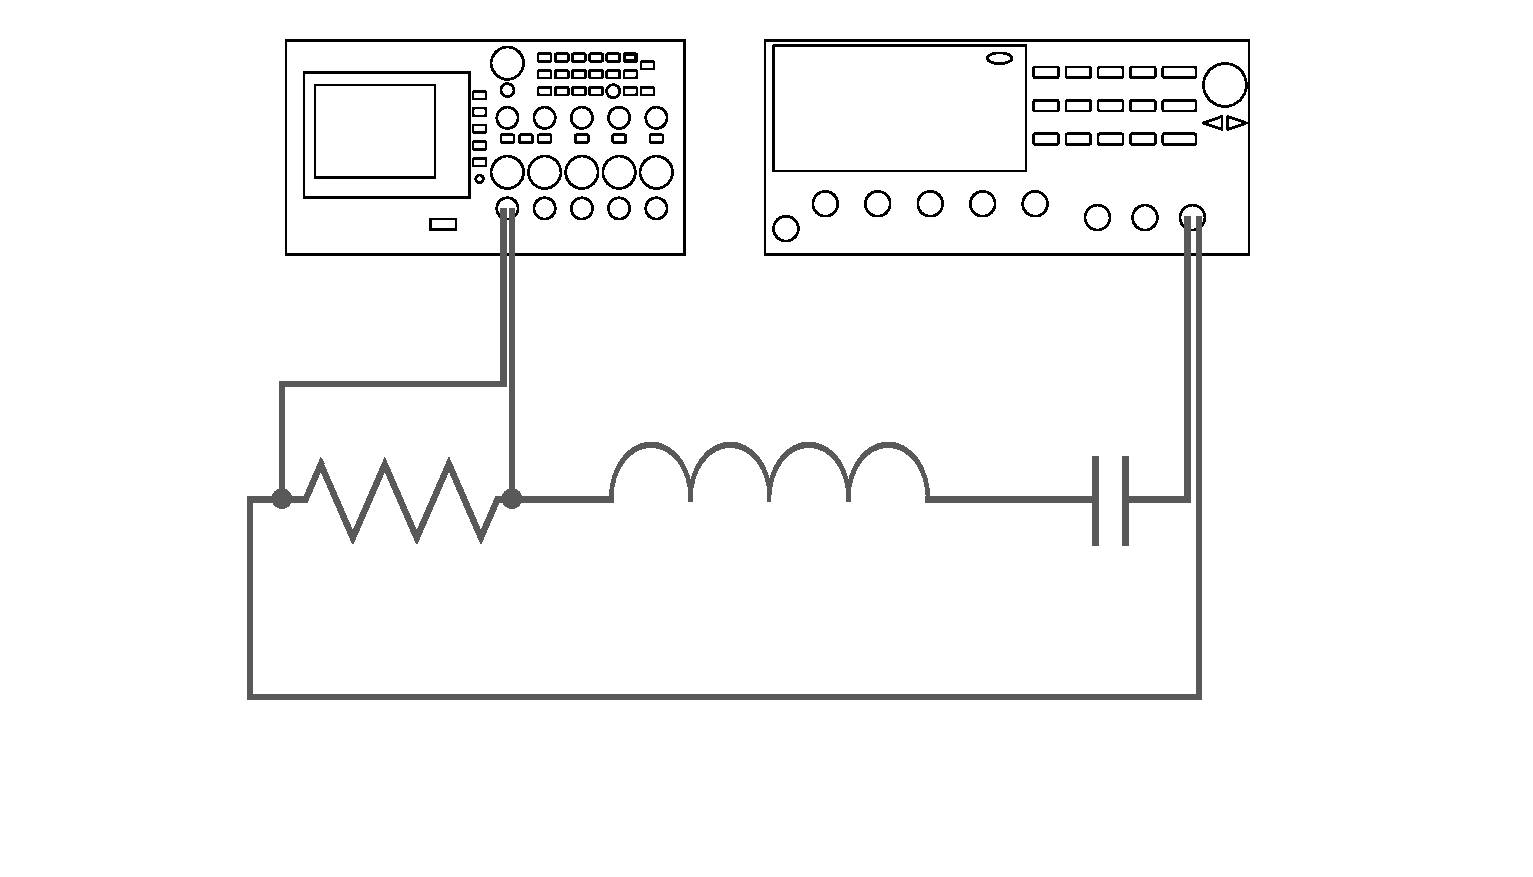
\includegraphics[width=8cm]{material/circuit.eps}
        \caption{回路図}
        \label{circuit}
    \end{center}
\end{figure}

\subsection{使用機器}
使用した機器は表\ref{device}に示す．
\begin{table}[htbp]
    \begin{center}
    \caption{使用機器}
    \label{device}
    \begin{tabular}{lrlll}
        \hline
        機器 & 個数$\mathrm{[個]}$ & 製造会社 & 型番号 & 補足\\ \hline
        \csvreader[late after line=\\]{material/device.csv}
        {name=\name,num=\num,co=\co,model=\model,note=\note}
        {\name & \num & \co & \model & \note}
        \hline
    \end{tabular}
    \end{center}
\end{table}

\subsection{使用素子}
使用した素子とその抵抗値，誘導係数，静電容量を表\ref{element}に示す．なお，O.L.は測定不能，即ち，測定範囲を超えてしまっていることを表し，N.R.はその値を計測しなかったことを表している．
\begin{table}[htbp]
    \begin{center}
    \caption{使用素子}
    \label{element}
    \begin{tabular}{l|rrr}
    % \begin{tabular}{l|D{.}{.}{2}D{.}{.}{4}r}
        \hline
        素子 & 抵抗値$R/\si{\ohm}$ & 誘導係数$L/\si{\milli\henry}$ & 静電容量 $C/\mathrm{nF} $\\ \hline
        \csvreader[late after line=\\]{material/elemout.csv}
        {elem=\elem,res=\res,rea=\rea,cap=\cap}
        {\elem & \res & \rea & \cap}
        \hline
    \end{tabular}
    \end{center}
\end{table}

第$1$に，抵抗器に抵抗器$1$を用いて臨界減衰に近い電圧波形を観察する．第$2$に，抵抗器に抵抗器$2$を用いて減衰振動する電圧波形を観察し，ピーク電圧と波形を記録した．第$3$に，抵抗器に抵抗器$3$を用いて過減衰を観察し，電圧の時間変化と波形を記録した．

\section{実験結果}

\subsection{臨界減衰}
最初は，後に示す図\ref{OD-shape}と似たような波形に大きくノイズが乗っていた．その後，各素子を接続し直すことでなめらかな波形が観察された．

\subsection{減衰振動}
観測された電圧$V_\mathrm{R}$の波形を図\ref{DO-shape}に示す．

\begin{figure}[htbp]
    \begin{center}
        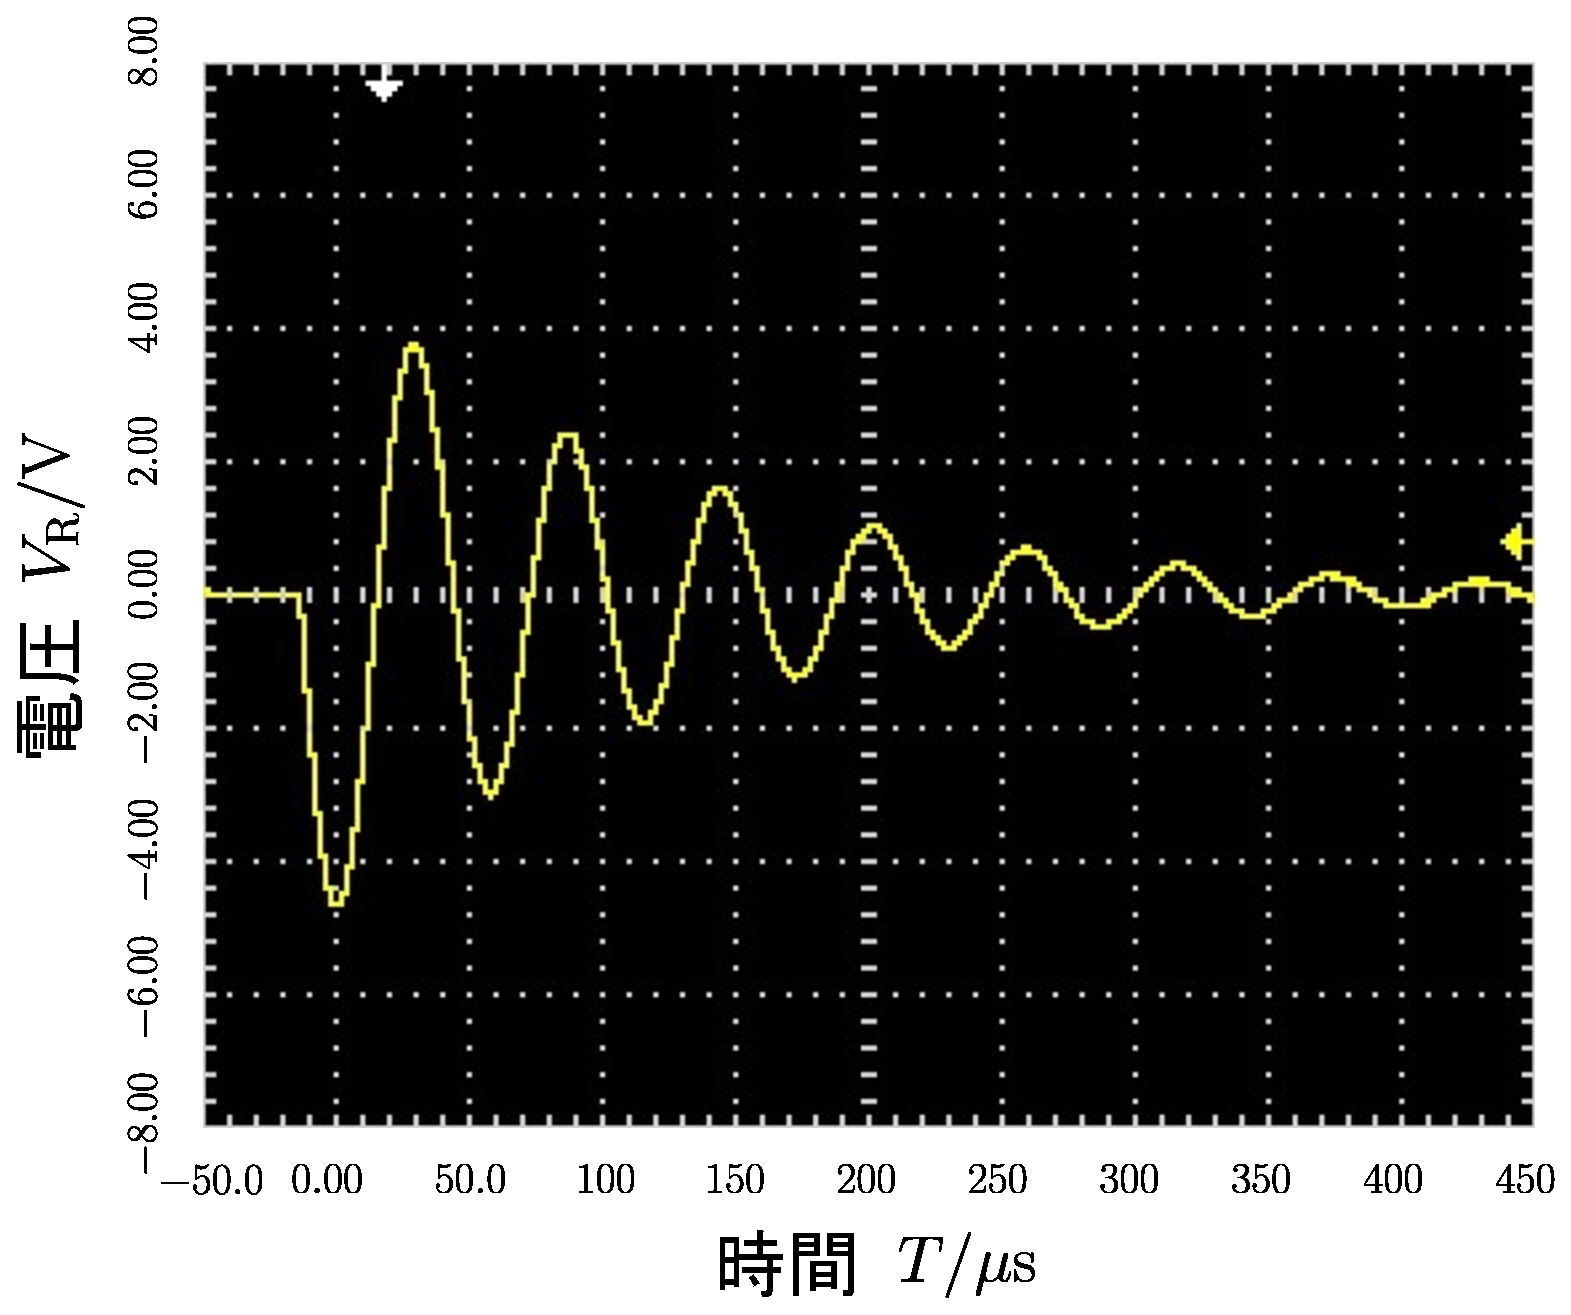
\includegraphics[width=10cm]{material/DOshape.eps}
        \caption{減衰振動の波形}
        \label{DO-shape}
    \end{center}
\end{figure}

$V_\mathrm{R}$の負のピーク電圧の変化を表\ref{DOtable}に示す．

\begin{table}[htbp]
    \begin{center}
        \caption{減衰振動における時間と電圧の関係}
        \label{DOtable}
        \begin{tabular}{r|r|r}
            \hline
            時間$t_n/\si{\second}$ & 電圧$V_n/\si{\volt}$ & 電圧比の対数$\ln\left( V_n/V_0 \right)$ \\ \hline
            \csvreader[late after line=\\]{material/DOout.csv}
            {time=\time,volt=\volt,lnR=\lnR}
            {\time & \volt & \lnR}
            \hline
        \end{tabular}
    \end{center}
\end{table}

図\ref{DO-graph}に電圧比の対数と時間のグラフを示す．
\begin{figure}[htbp]
    \begin{center}
        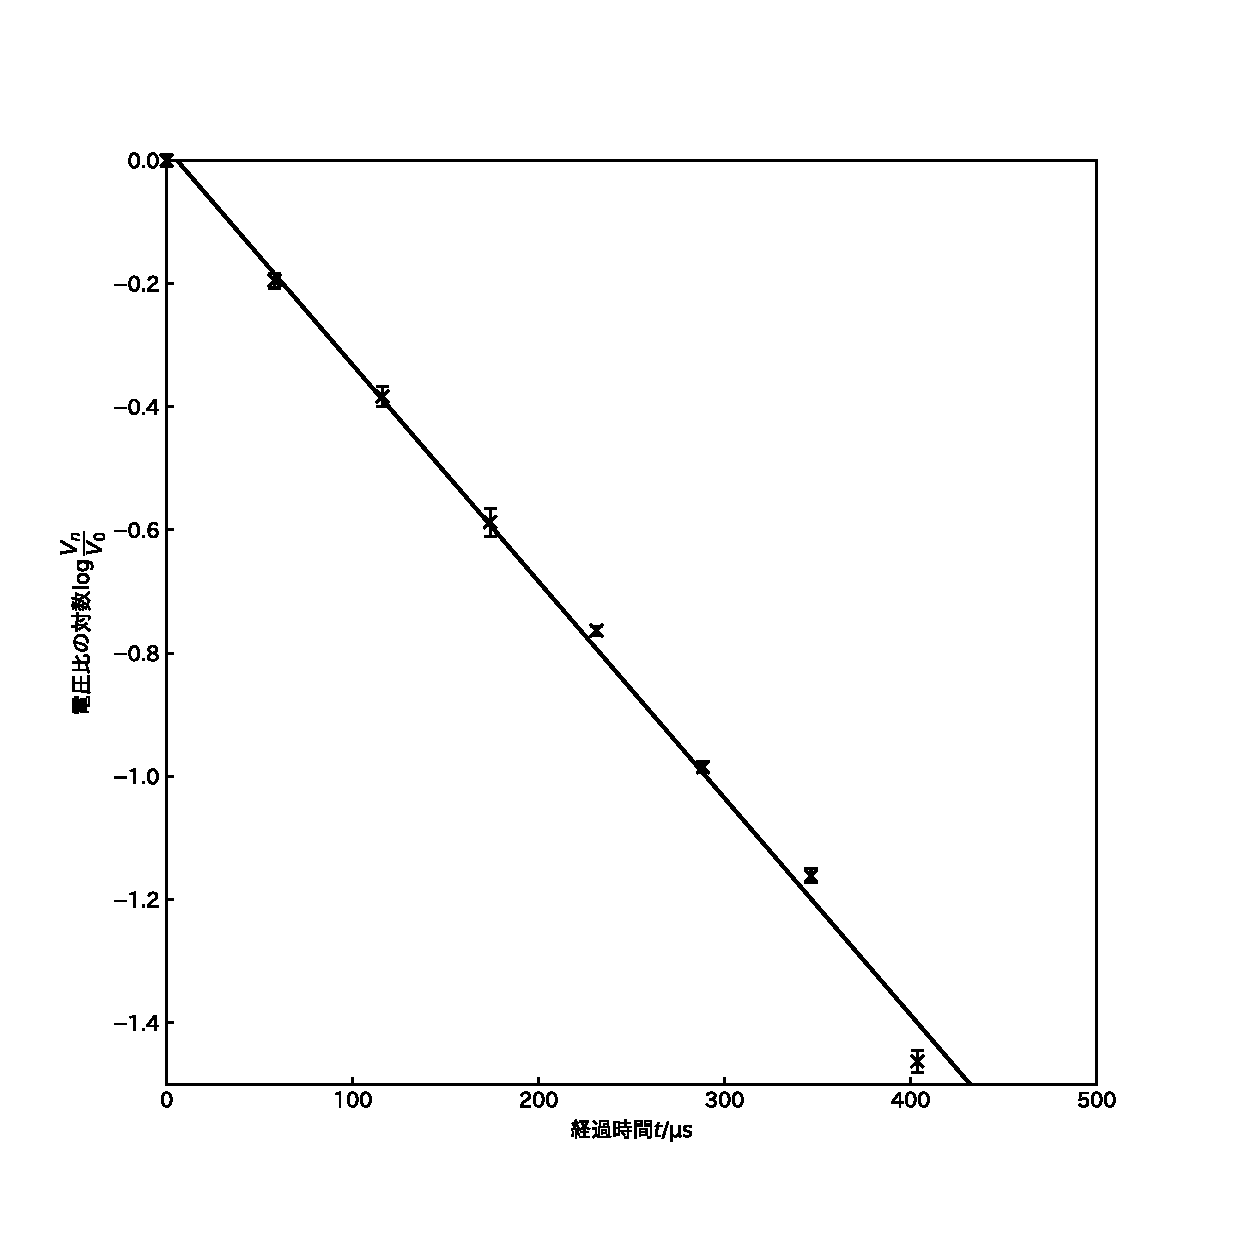
\includegraphics[width=10cm]{material/DOgraph.eps}
        \caption{電圧比の対数と時間の関係}
        \label{DO-graph}
    \end{center}
\end{figure}

\subsection{過減衰}

観測された電圧$V_\mathrm{R}$の波形を図\ref{OD-shape}に示す．

\begin{figure}[htbp]
    \begin{center}
        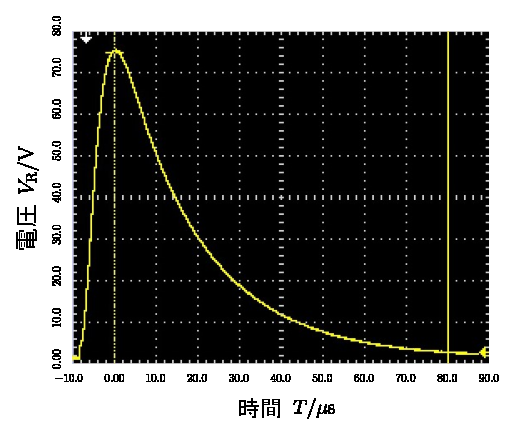
\includegraphics[width=10cm]{material/ODshape.eps}
        \caption{減衰振動の波形}
        \label{OD-shape}
    \end{center}
\end{figure}

$V_\mathrm{R}$の電圧の変化を表\ref{ODtable}に示す．
\begin{table}[htbp]
    \begin{center}
        \caption{過減衰における時間と電圧の関係}
        \label{ODtable}
        \begin{tabular}{r|r|r}
            \hline
            時間$t_n/\si{\second}$ & 電圧$V_n/\si{\volt}$ & 電圧比の対数$\ln\left( V_n/V_0 \right)$ \\ \hline
            \csvreader[late after line=\\]{material/ODout.csv}
            {time=\time,volt=\volt,lnR=\lnR}
            {\time & \volt & \lnR}
            \hline
        \end{tabular}
    \end{center}
\end{table}

図\ref{OD-graph}に電圧比の対数と時間のグラフを示す．
\begin{figure}[htbp]
    \begin{center}
        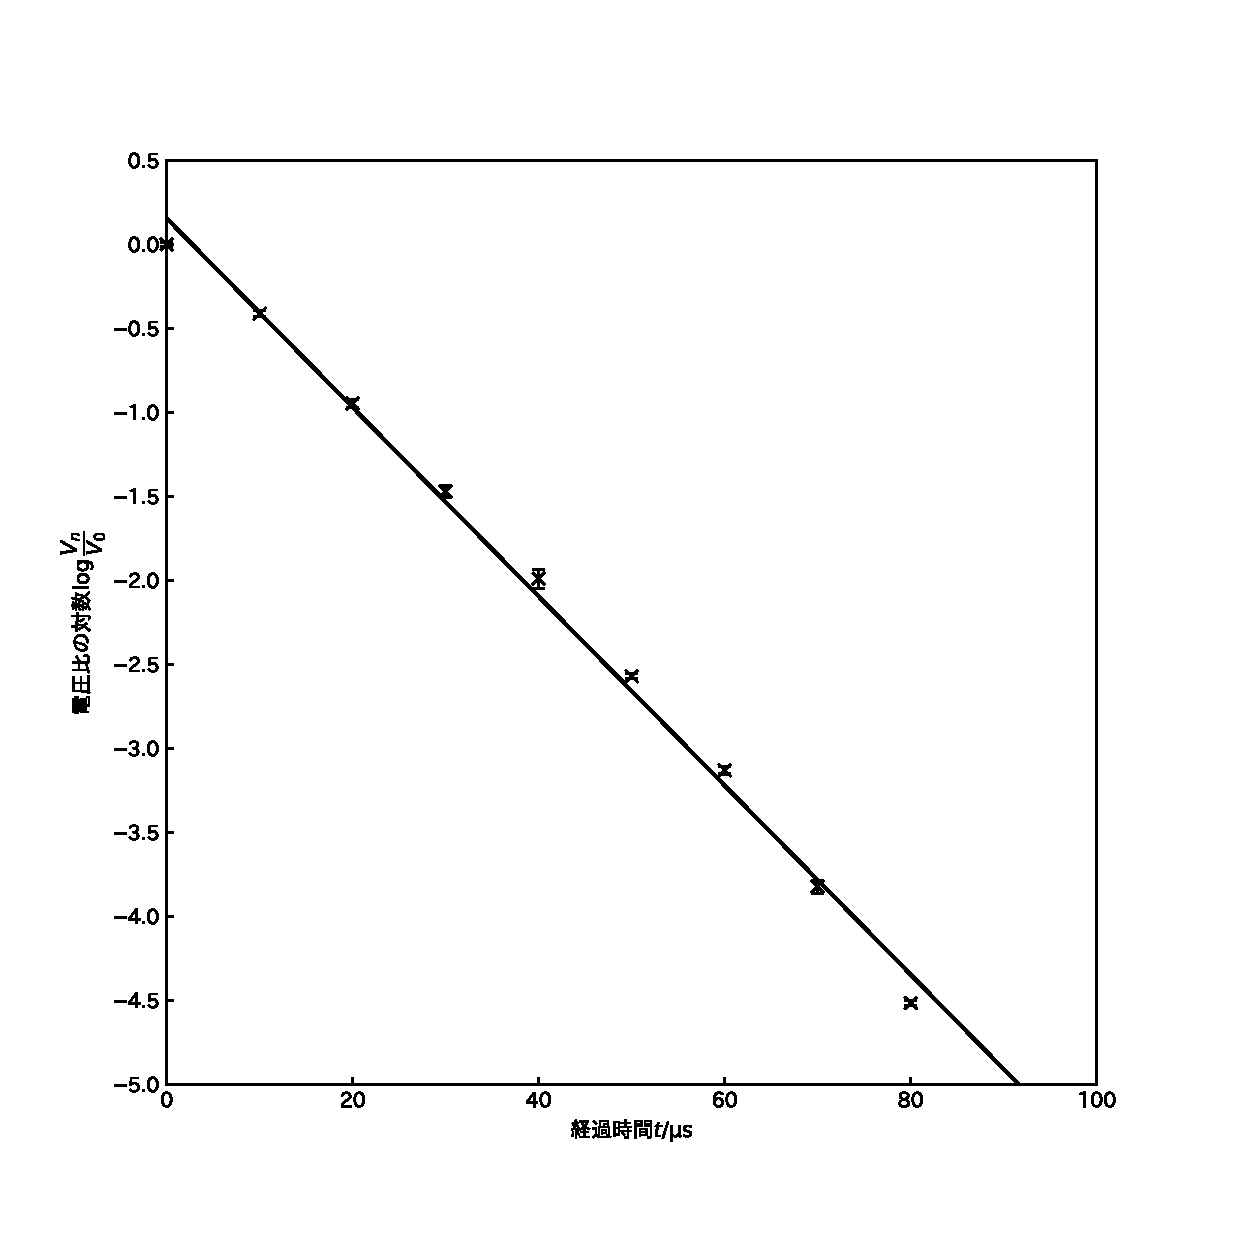
\includegraphics[width=10cm]{material/ODgraph.eps}
        \caption{電圧比の対数と時間の関係}
        \label{OD-graph}
    \end{center}
\end{figure}

\section{考察}

\subsection{抵抗値の変化に依る電流の振る舞い}
まず，抵抗値がごく小さいときを考える．例えば，理想的に$R=0$のときには$\gamma=0$となり，\ref{sec:DO}減衰振動で議論したように電流は減衰振動する．また，抵抗値をだんだん大きくしていくと，$\gamma$が大きくなり，$\omega'$が小さくなることから，この減衰振動の周期が長くなっていく．次に，抵抗値が，$\gamma$が$\omega$に近くなるような値をとるときを考える．例えば，理論的に$\gamma=\omega$のときは\ref{sec:LD}臨界減衰で議論したように電流は振る舞うが，これは周期が限りなく大きい減衰振動ととらえることもできる．次に抵抗値がさらに大きくなると，\ref{sec:OD}過減衰で議論したように電流は過減衰する．また，抵抗値をだんだん大きくしていくと，$\gamma$が大きくなり，$\omega'$が大きくなることから

\subsection{考慮できていない回路定数}
表\ref{element}の回路定数の中で観測しなかった量（N.R.）が含まれない抵抗値$R$を最も信頼できる値と見做して，これを基準に誘導係数と静電容量について，理論的には考慮できていないが，実験的には観測される分を算出する．ここで，抵抗値$R$と実験で得られる$\gamma_\mathrm{exp}$，$\omega_\mathrm{exp}$を既知であるとすると，実験的に観測される誘導係数$L_\mathrm{exp}$と静電容量$C_\mathrm{exp}$は，
\begin{align}
    L_\mathrm{exp} &= \frac{R}{2\gamma_\mathrm{exp}} & C_\mathrm{exp} = \frac{2\gamma_\mathrm{exp}}{\omega^2 R}
\end{align}
と表される．

\begin{thebibliography}{99}
    \bibitem{LCR} AD-5826/AD-5827 LCR メータ，取扱説明書ダウンロード | サポート | 株式会社エー・アンド・デイ，株式会社エー・アンド・デイ　A\&D Company, Limited，株式会社エー・アンド・デイ，2023-06-28閲覧，\url{https://www.aandd.co.jp/pdf_storage/manual/sp/m_ad5826_ad5827.pdf}．
    \bibitem{DMM} ハンディタイプ　デジタル・マルチメータ VOAC21 - 岩崎通信機株式会社，電子計測機器／電子部品 | 岩崎通信機株式会社，岩崎通信機株式会社，2023-06-28閲覧，\url{https://www.iti.iwatsu.co.jp/ja/products/voac/13_17.html}．
    \bibitem{Oscillo} TDS2000C Digital Storage Oscilloscope Datasheet，半導体・電子部品代理店 - マウザー・エレクトロニクス Mouser Electronics 日本，Mouser Electronics，2023-06-28閲覧，\url{https://www.mouser.jp/datasheet/2/403/TDS2000C_Digital_Storage_Oscilloscope_Datasheet_3G-2308159.pdf}．
    \bibitem{FG} C3C4SFG-2000Series，Home-GW Instek，GW Instek，2023-06-28閲覧，\url{https://www.gwinstek.com/en-global/products/downloadSeriesDownNew/12786/478}．
\end{thebibliography}

\end{document}